\section{Consensus}
\label{sec:consensus}

\pgfplotsset{consensusAxisBasicStyle/.style={
	axis lines = center,
	scaled x ticks = false,
	scaled y ticks = false,
	legend columns = 3,
	xmin = 0,
	height = 5cm,
	width=(4 * \textwidth) / 5,
}}

\pgfplotsset{consensusAxisEvStyle/.style={
	consensusAxisBasicStyle,
	xlabel = P,
	ylabel = EV,
	ymin = -150,
	ymax = 150,
}}

\nemquote{%
You know what, sometimes it seems to me we’re living in a world that we fabricate for ourselves.
We decide what’s good and what isn’t, we draw maps of meanings for ourselves...
And then we spend our whole lives struggling with what we have invented for ourselves.
The problem is that each of us has our own version of it, so people find it hard to understand each other.
}{Olga Tokarczuk}

\nemchapterfirstletter{B}{yzantine} consensus is a key problem faced by all decentralized systems.
Essentially, the crux of the problem is finding a way to get independent actors to cooperate without cheating.
Bitcoin's key innovation was a solution to this problem that is based on Proof of Work (PoW).
After each new block is accepted into Bitcoin's main chain, all miners begin a competition to find the next block.
All miners are incentivized to extend the main chain instead of forks because the chain with the greatest cumulative hashing power is the reference chain.
Miners calculate hashes as quickly as possible until one produces a candidate block with a hash below the current network difficulty target.
A miner's probability of mining a block is proportional to the miner's hash rate relative to the network's total hash rate.
This necessarily leads to a computational arms race and uses a lot of electricity.

Proof of Stake (PoS)\cite{King:2012:PPP}\cite{Nxt2013} blockchains were introduced after Bitcoin.
They presented an alternative solution to the Byzantine consensus problem that did not require significant power consumption.
Fundamentally, these chains behaved similarly to Bitcoin with one important difference.
Instead of predicating the probability of creating a block on a node's relative hash rate, the probability is based on a node's relative stake in the network.
Since richer accounts are able to produce more blocks than poorer accounts, this scheme tends to allow the rich to get richer.

\codenamespace uses a modified version of PoS that borrows key concepts from Proof of Importance (PoI).
This new weighting attempts to capture the original intent of PoI, which was to award \emph{users} preferentially relative to \emph{hoarders}, but not suffer from the scaling issues inherent in the original PoI algorithm.

There are multiple factors that contribute to a healthy ecosystem.
All else equal, accounts with larger stakes making more transactions and running nodes have more skin in the game and should be rewarded accordingly.
Firstly, accounts with larger balances have larger stakes in the network and have greater incentives to see the ecosystem as a whole succeed.
The amount of the currency an account owns is a measure of its stake.
Secondly, accounts should be encouraged to use the network by making transactions.
Network usage can be approximated by the total amount of fees paid by an account.
Thirdly, accounts should be encouraged to run nodes to strengthen the network.
This can be approximated by the number of times an account is the beneficiary of a block
\footnote{
	This measure is strongly correlated with stake when all accounts are actively running nodes.
	Its intent is to differentiate accounts running nodes from accounts idling.
}.
Since the node owner has complete control over defining its beneficiary, any benevolent node owner can alternatively boost this measure for a third-party.

Importances are recalculated every \nemsetting{network}{importanceGrouping} blocks.
This reduces the pressure on the blockchain because the importance calculation is relatively expensive and processing it every block would be prohibitive.
Additionally, recalculating importances periodically allows for automatic state aging.
Overall, it is beneficial to calculate importances periodically rather than every block.

In order to encourage good behavior, accounts active in an older time period should not obtain an eternal advantage due to their previous virtuous behavior.
Instead, importance boosts granted by transaction and node scores are time limited.
The boost lasts for five \nemsetting{network}{importanceGrouping} intervals.

\subsection{Weighting Algorithm}
\label{sec:consensus:weighting}

All accounts that have a balance of at least \nemsetting{network}{minHarvesterBalance} participate in the importance calculation and are called \emph{high value accounts}.
Notice that this set of accounts is a superset of the set of accounts eligible for block generation \nemrefparens{sec:blockchain:generation}.
In other words, a nonzero importance at the most recent importance recalculation is a necessary but not sufficient condition for block generation.

An account's \emph{importance score} is calculated by combining three component scores: stake, transaction and node.

The stake score, $S_A$, for an account $A$ is the percentage of currency it owns relative to the total currency owned by all high value accounts.
This percentage is no less than the percentage of currency the account owns relative to all outstanding currency.
Let $B_A$ represent the amount of currency owned by account $A$.
The stake score for account $A$ is calculated for each eligible account as follows:

\begin{equation}
S_A = \frac{B_A}{\sum\limits_{\substack{a \in \mathname{high value accounts}}} B_a}
\end{equation}

The transaction score, $T_A$, for an account $A$ is the percentage of transaction fees it has paid relative to all fees paid by high value accounts within a time period $P$.
Let $\mathfunc{FeesPaid}{A}$ represent the amount of fees paid by $A$ in the time period $P$.
The transaction score for account $A$ is calculated for each eligible account as follows:

\begin{equation}
T_A = \frac{\mathfunc{FeesPaid}(A)}{\sum\limits_{\substack{a \in \mathname{high value accounts}}} \mathfunc{FeesPaid}(a)}
\end{equation}

The node score, $N_A$, for an account $A$ is the percentage of times it has been specified as a beneficiary relative to the total number of high value account beneficiaries within a time period $P$.
Let $\mathfunc{BeneficiaryCount}{A}$represent the number of times $A$ has been specified as a beneficiary in the time period $P$.
The node score for account $A$ is calculated for each eligible account as follows:

\begin{equation}
N_A = \frac{\mathfunc{BeneficiaryCount}(A)}{\sum\limits_{\substack{a \in \mathname{high value accounts}}} \mathfunc{BeneficiaryCount}(a)}
\end{equation}

Together, the transaction and node scores are called the \emph{activity score} because they are both dynamic and derived from an account's activity as opposed to its stake.
The transaction score is weighted at 80\% and the node score at 20\%.
Additionally, the combined score is scaled relative to an account's balance so that there is a dampening effect of activity on importance as stake increases
\footnote{The activity score is rescaled after dampening so that it contributes the desired \nemsetting{network}{importanceActivityPercentage} to the importance calculation.}.
This effectively allows active smaller accounts to gain an outsized boost relative to active larger accounts.
This partially redistributes importance away from rich accounts towards poorer accounts and somewhat counteracts the rich getting richer phenomenon inherent in PoS.
The prominence of activity relative to stake can be configured by \nemsetting{network}{importanceActivityPercentage}.
When this value is zero, \codenamespace behaves like a pure PoS blockchain.
Setting this to too a high value could weaken blockchain security by lowering the cost for an attacker to obtain majority importance and execute a 51\% attack.

As a performance optimization, activity information is only collected for accounts that are \emph{high value} at the time of the most recent importance calculation.
Between importance recalculations, new data is stored in a working bucket.
At each importance recalculation, existing buckets are shifted, the working bucket is finalized and a new working bucket is created.
Each bucket influences at most five importance recalculations.
As a result, activity information quickly expires.

\begin{figure}[ht]
	\nemcenterwithcaption{
		\begin{tikzpicture}[node distance=0.2cm and 0.5cm]
			\node[anchor=center] (lbl1) {buckets};
			\node[crecb,right=of lbl1] (bucket1) {\texttt{1}};
			\node[crecb,right=of bucket1] (bucket2) {\texttt{2}};
			\node[crecb,right=of bucket2] (bucket3) {\texttt{3}};
			\node[crecb,right=of bucket3] (bucket4) {\texttt{4}};
			\node[crecb,right=of bucket4] (bucket5) {\texttt{5}};
			\node[crecb,right=of bucket5] (bucket6) {\texttt{6}};
			\node[crecb,right=of bucket6] (bucket7) {\texttt{7}};
			\node[crecb,right=of bucket7] (bucket8) {\texttt{8}};
			\node[crecb,right=of bucket8] (bucket9) {\texttt{9}};
			\node[crecb,right=of bucket9] (bucketW) {\texttt{W}};

			\draw[decorate,decoration={brace,mirror},very thick]
				([yshift=-4pt] bucket1.south west)
				-- node[below] (xd1) {bucket group 5}
				([yshift=-4pt] bucket5.south east);

			\draw[decorate,decoration={brace,mirror},very thick]
				([yshift=-20pt] bucket2.south west)
				-- node[below] {bucket group 6}
				([yshift=-20pt] bucket6.south east);

			\draw[decorate,decoration={brace,mirror},very thick]
				([yshift=-36pt] bucket3.south west)
				-- node[below] {bucket group 7}
				([yshift=-36pt] bucket7.south east);

			\draw[decorate,decoration={brace,mirror},very thick]
				([yshift=-52pt] bucket4.south west)
				-- node[below] {bucket group 8}
				([yshift=-52pt] bucket8.south east);

			\draw[decorate,decoration={brace,mirror},very thick]
				([yshift=-68pt] bucket5.south west)
				-- node[below] {bucket group 9}
				([yshift=-68pt] bucket9.south east);
		\end{tikzpicture}
	}{Activity buckets}
\end{figure}

The \nemsetting{network}{totalChainImportance} setting specifies the total importance that is distributed among all accounts in a network.
Given that, the spot importance of the account $A$, $I'_A$, can be calculated as follows
\footnote{
	There is some additional edge case handling that is not reflected in the equation around how zero component scores are handled.
	If either the transaction or node scores is zero, the other will be scaled up and serve as the fully weighted activity score.
	If both are zero, the stake score will be scaled up and used exclusively.
}:
\begin{align*}
	\gamma = \: & \nemsetting{network}{importanceActivityPercentage} \\
	\mathvar{ActivityScore}'_A = \: & \frac{\nemsetting{network}{minHarvesterBalance}}{B_A} \cdot \left( 0.8 \cdot T_A + 0.2 \cdot N_A \right) \\
	\mathvar{ActivityScore}_A = \: & \frac{ActivityScore'_A}{\sum\limits_{\substack{a \in \mathname{high value accounts}}} ActivityScore'_a} \\
	I'_A = \: & \nemsetting{network}{totalChainImportance} \cdot \left( \left(1 - \gamma \right) \cdot S_A + \gamma \cdot ActivityScore_A \right)
\end{align*}

The final importance score, $I_A$ for account $A$ is calculated as the minimum of $I'_A$ at the current and previous importance calculations.
This serves as a precaution against a stake grinding attack and a general incentive to minimize unnecessary stake movement.
There is no rescaling, so the sum of $I_A$ for all high value accounts might be less than \nemsetting{network}{totalChainImportance}.

\subsection{Sybil Attack}
\index{sybil attack}

A \emph{Sybil attack} on a peer-to-peer network occurs when an attacker creates multiple identities in order to gain a disproportionately large influence over the network or some other advantage.
In \codename, an attacker might attempt such an attack to boost importance.
Each component of the importance score needs to be robust against such attacks.

As described in \nemref{sec:consensus:weighting}, an account's activity score is dampened relative to its balance.
Accordingly, splitting an account's balance among multiple accounts will lower the average dampening factor applied.
Assuming a constant level of activity is \emph{sustained} before and after redistribution, the cumulative importance will be higher post split
\footnote{
	This assumes that only one account splits.
	The effect is lessened when multiple accounts split because activity scores are relative.
}.
This effect is by design and encourages virtuous behavior because the importance boost is only realized if activity is sustained.
Preservation of the transaction score encourages transacting and paying fees from multiple accounts.
Preservation of the node score encourages running additional nodes and connecting them to the network.

Assume $\mu := \nemsetting{network}{minHarvesterBalance}$ and an attacker that owns $N \cdot \mu$ total currency.
Consider two extremes:

\begin{enumerate}
	\item{The attacker has a single account with $N \cdot \mu$ currency.}
	\item{The attacker has $N$ accounts with $\mu$ currency.}
\end{enumerate}

\subsubsection*{Boosting Stake Score}

In both extremes, the total currency owned by the attacker is the same.
Accordingly, the stake score is the same and there is no benefit gained from splitting accounts.
For emphasis:

\begin{equation}
B_A = \sum\limits_{a \in \{1, \dotso, N\}} B_a
\end{equation}

\subsubsection*{Boosting Node Score}

\codenamespace allows a node owner to specify a beneficiary for every block harvested on their node.
Each time an account is specified as a beneficiary, assuming it is already a \emph{high value account}, it will get a slight boost in its node score.

In both extremes, the total beneficiary count for the attacker is the same.
Accordingly, the node score is the same and there is no undeserved benefit gained from splitting accounts.
For emphasis:

\begin{equation}
\mathfunc{BeneficiaryCount}(A) = \sum\limits_{a \in \{1, \dotso, N\}} \mathfunc{BeneficiaryCount}(a)
\end{equation}

The attacker might obtain a higher node score if running more nodes allows the attacker's nodes to host more delegated harvesters.
This is not a bad outcome and by design.
It encourages more nodes in the network, which is a good thing that strengthens the network.

The attacker could try to cheat by setting up $N$ virtual nodes pointing to a single physical machine.
Each of these virtual nodes would be treated by the rest of the network as a normal node, and the underlying physical node would be interacted with $N$ times more often than a normal node in the network.
This implies that the virtual nodes are running on a strong physical server, which is still beneficial to the network relative to a weaker physical server.

\subsubsection*{Boosting Transaction Score}

The transaction score is solely based on fees.
There is no difference between one huge account spending $X$ on fees and $N$ smaller accounts, each spending $\frac{X}{N}$ on fees.
For emphasis:

\begin{equation}
\mathfunc{FeesPaid}(A) = \sum\limits_{a \in \{1, \dotso, N\}} \mathfunc{FeesPaid}(a)
\end{equation}

The only possibility to boost transaction score is a \emph{fee attack}, which is discussed in detail in \nemref{sec:consensus:feeAttack}.

\subsection{Nothing at Stake Attack}

A general criticism of PoS consensus is the \emph{nothing at stake} attack.
This attack theoretically exists when the opportunity cost of creating a block is negligible.
There are two variations of this attack.

In the first variation, all harvesters except the attacker harvest on all forks.
Simplifying the description to assume a binary fork, the attacker would submit a payment to one branch and immediately start harvesting on the other branch.
Assuming the attacker has sufficient importance to harvest blocks, eventually the branch without the attacker's payment will become the reference chain because it will have a higher score
\footnote{This assumes that there is only a single attacker or all attackers collude to withhold harvesting from the same branch.}.
The attacker's payment is not included in this branch, so the attacker's funds are effectively returned.

There are three primary defenses against this attack.
First, the attacker has a limited amount of time to produce a better chain because at most \nemsetting{network}{maxRollbackBlocks} blocks can be rolled back.
If the merchant waits to render services until at least this many blocks are confirmed, the attack is impossible.
Second, in order to execute a successful nothing at stake attack, the attacker must own a significant importance in the network
\footnote{
	Theoretically, an attacker would need just \nemsetting{network}{minHarvesterBalance} to execute this attack.
	In practice, in order to guarantee successful execution, the attacker would need a large enough importance to always harvest a block within the rollback interval.
}.
Third, successful execution of this attack against the network will likely have a negative influence on the currency value.
Since other harvesters, by harvesting on all forks, enable this attack, profit-maximizing harvesters should only harvest on a single chain to preclude it.

In the second variation, a single attacker harvests on all forks and attempts to capture all fees irrespective of which chain becomes the reference chain.
An attacker could harvest on all forks starting from the second block searching for the chain in which the attacker has harvested the most fees.
Since block acceptance is probabilistic, in theory, an attacker could spend infinite time building the perfect chain in which the attacker has harvested all blocks.

Most theoretical nothing at stake attacks imagine an idealized blockchain and ignore protocol-level safeguards that protect against such attacks.
In practice, this type of attack is impractical if the attacker owns a minority of currency.
The aforementioned two defenses are also applicable here.
In addition, changes in block difficulty \nemrefparens{sec:blockchain:difficulty} are capped at 5\%.
It will take some time for the difficulty of the attacker's chain to adjust downward, which will cause the block times at the beginning of the secret chain to significantly lag those of the main chain.
These large time differences will make it unlikely for the attacker to produce a chain with a better score \nemrefparens{sec:blockchain:score}.

A small amount of stake aging also decreases the likelihood of this second variation.
Requiring accounts to have nonzero importances for two consecutive importance recalculations as a precondition for harvesting makes generation hash grinding\footnote{This is an attempt to brute force the block hit \nemrefparens{sec:blockchain:generation}, which is dependent on generation hash.} attacks nonviable.
In order to exploit this, the attacker would need to move all currency to a specific account more than \nemsetting{network}{importanceGrouping} blocks before the attack could be carried out.
Since the attacker can't know all the blocks that will be confirmed in the intervening period, such movement cannot result in any benefit.

\subsection{Fee Attack}
\label{sec:consensus:feeAttack}

A \emph{fee attack} is an attempt by an attacker to exploit the transaction score by paying large fees in order to boost its own importance.
The attack is considered effective if it yields a positive expected value.

The analysis in this section will be performed using the recommended public network settings.
These include \nemsetting{network}{totalChainImportance} equal to 9 billion, \nemsetting{network}{importanceGrouping} equal to 359 blocks and \nemsetting{minHarvesterBalance} equal to 10000 currency.
Additionally, \nemsetting{network}{importanceActivityPercentage} is 5, so the cumulative transaction score accounts for 4\% of importance.

\subsubsection*{Large Account}

Consider an account that is large enough to harvest one block per importance recalculation interval without any activity boosting.
Assuming only 2 of 9 billion currency is actively harvesting, the account will need at least 5.57 million currency to harvest this frequently.

The account might try to make a profit by adding a transaction with a high fee to one of its own harvested blocks each recalculation interval.
This would boost the account's importance and allow it to harvest more blocks in the future and, consequently, collect more fees.
However, this activity is not risk free.
The account risks paying the high fee if a better block replaces its block.
When the original block is unwound, the high fee transaction will enter the unconfirmed transactions cache and be eligible for inclusion in a new block created by a different harvester.
This scenario is a net loss because the account will have to pay the high fee.

Let $P$ be the probability of a fork resulting in a loss, $F$ be the high fee in a block, and $\bar{F}$ be the average fee in a block.
The expected value, $EV$, can be approximated as follows:
\begin{align*}
	\tag{importance boost}\beta &= 0.04 \cdot \frac{1}{557} \cdot \frac{F}{359 \cdot \bar{F} + F} \\
	\tag{expected value} EV &= \beta \cdot \frac{359}{P} \cdot \bar{F} - F
\end{align*}

The expected value is positive for small values of $P$.
As $P$ or $F$ increases, it quickly becomes negative.
Using the recommended public network settings, $P$ needs to be less than 0.0001 for the expected value to be positive.
This implies a fork resulting in a loss occurs less than once every 10000 blocks.
Given the mechanism of distributed consensus, this is a near impossibility.
Small one or two block forks occur quite frequently.

\begin{figure}[H]
	\nemcenterwithcaption{
		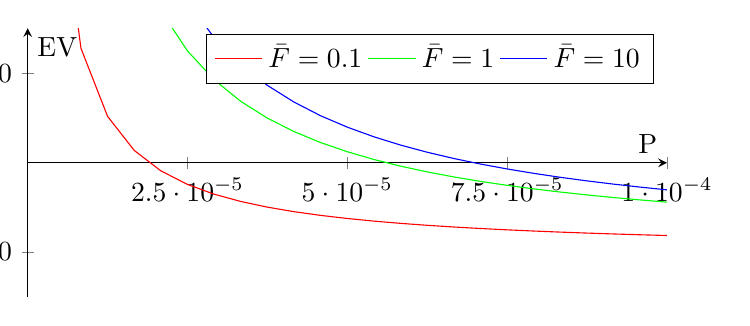
\begin{tikzpicture}[trim axis left]
			\begin{axis}[consensusAxisEvStyle, xtick distance=0.000025, xmax = 0.0001]
				\addplot[color=red,domain=0:0.0001]{(0.04 / 557 * 100 / (359 * 0.1 + 100)) * (359 / x) * 0.1 - 100};
				\addlegendentry{$\bar{F} = 0.1$}

				\addplot[color=green,domain=0:0.0001]{(0.04 / 557 * 100 / (359 * 1 + 100)) * (359 / x) * 1 - 100};
				\addlegendentry{$\bar{F} = 1$}

				\addplot[color=blue,domain=0:0.0001]{(0.04 / 557 * 100 / (359 * 10 + 100)) * (359 / x) * 10 - 100};
				\addlegendentry{$\bar{F} = 10$}
			\end{axis}
		\end{tikzpicture}
	}{Fee attack large account analysis (F = 100)}
\end{figure}

\subsubsection*{Small Account}

Consider an account that has a balance equal to \nemsetting{network}{minHarvesterBalance}.
Assume the account makes one transaction with high fees in two consecutive recalculation intervals.
These fees are lost to other harvesters because the probability of the account harvesting a block is quite small.
The high fees paid boost the account’s importance enough so that it is able to harvest at least one block per importance recalculation interval.
From this point forward, the account behaves like the large account in the previous section.
It will also add a transaction with a high fee to one of its own harvested blocks each recalculation interval.
The account hopes that due to the increased probability of harvesting a block, its additional collected fees will exceed its costs.

\begin{figure}[H]
	\nemcenterwithcaption{
		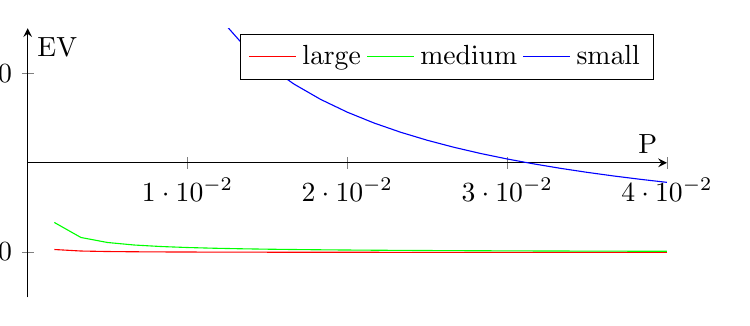
\begin{tikzpicture}[trim axis left]
			\begin{axis}[consensusAxisEvStyle, xtick distance=0.01, xmax = 0.04]
				\addplot[color=red,domain=0:0.04]{(0.04 / 557 * 100 / (359 * 1 + 100)) * (359 / x) * 1 - 100};
				\addlegendentry{large}

				\addplot[color=green,domain=0:0.04]{(0.04 / 56 * 100 / (359 * 1 + 100)) * (359 / x) * 1 - 100};
				\addlegendentry{medium}

				\addplot[color=blue,domain=0:0.04]{(0.04 * 100 / (359 * 1 + 100)) * (359 / x) * 1 - 100};
				\addlegendentry{small}
			\end{axis}
		\end{tikzpicture}
	}{Fee attack balance sensitivity (F = 100, $\bar{F} = 1$)}
\end{figure}

Let $P$ be the probability of a fork resulting in a loss, $F$ be the high fee in a block, and $\bar{F}$ be the average fee in a block.
The expected value, $EV$, excluding the initial transaction fees, can be approximated as follows\footnote{
The difference relative to the large account example is that the damping factor is completely removed.}:
\begin{align*}
	\tag{importance boost}\beta &= 0.04 \cdot \frac{F}{359 \cdot \bar{F} + F} \\
	\tag{expected value} EV &= \beta \cdot \frac{359}{P} \cdot \bar{F} - F
\end{align*}

The expected value is positive for larger values of $P$ than in the large account scenario.
A fee attack confers an outsized benefit to a small account relative to a large account because the activity scores of the latter are dampened more aggressively than those of the former.
Specifically, a damping factor of $\frac{1}{557}$ is applied to the large account's activity score, but no damping factor is applied to the small account's activity score.

The expected value increases as $\bar{F}$ increases.
As $P$ or $F$ increases, it quickly becomes negative.
Using the recommended public network settings, $P$ needs to be less than 0.05 for the expected value to be positive.
This implies a fork resulting in a loss occurs less than once every 20 blocks.
Given the mechanism of distributed consensus, this is possible.

\begin{figure}[H]
	\nemcenterwithcaption{
		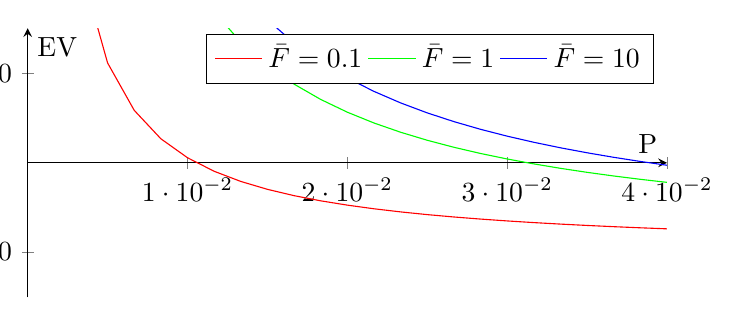
\begin{tikzpicture}[trim axis left]
			\begin{axis}[consensusAxisEvStyle, xtick distance=0.01, xmax = 0.04]
				\addplot[color=red,domain=0:0.04]{(0.04 * 100 / (359 * 0.1 + 100)) * (359 / x) * 0.1 - 100};
				\addlegendentry{$\bar{F} = 0.1$}

				\addplot[color=green,domain=0:0.04]{(0.04 * 100 / (359 * 1 + 100)) * (359 / x) * 1 - 100};
				\addlegendentry{$\bar{F} = 1$}

				\addplot[color=blue,domain=0:0.04]{(0.04 * 100 / (359 * 10 + 100)) * (359 / x) * 10 - 100};
				\addlegendentry{$\bar{F} = 10$}
			\end{axis}
		\end{tikzpicture}
	}{Fee attack small account analysis (F = 100)}
\end{figure}

\subsubsection*{Further Discussion}

Although a single small account can obtain a positive expected value by executing this attack, the payoff decreases as multiple accounts attempt it simultaneously.
Since there is a positive expected value, profit maximizing actors should all attempt this attack.
As more accounts attempt it, the importance boost obtained by each individual account decreases rapidly and, consequently, the expected value also decreases.\footnote{
	As more accounts produce high fee transactions to attempt this attack, $\bar{F}$ increases.
	For large numbers of attackers, if $F$ is not raised in proportion, the expected value of the attack can increase even though the importance boost per account decreases.
	This is an expected outcome since the value of blocks also increases significantly.
}.

Additionally, there is an upper limit on the number of small accounts that can execute this attack simultaneously.
In order for this attack to be successful, an account needs to be able to harvest at least one block per importance recalculation interval.
This presupposes the small account can boost its importance score by exploiting the transaction score component.
There is a theoretical limit on the number of accounts that can achieve a significant enough boost because both the importance allotted to the transaction score and the recalculation interval are finite.
Considering the recommended public network settings, this limit is approximately $0.04 \div \frac{1}{359} \approx 14.36$ accounts.

Let $N$ be the number of small accounts attempting the attack, $P$ be the probability of a fork resulting in a loss, $F$ be the high fee in a block, and $\bar{F}$ be the average fee in a block.
The expected value, $EV$, can be approximated as follows:
\begin{align*}
	\tag{importance boost}\beta &= 0.04 \cdot \frac{F}{359 \cdot \bar{F} + N \cdot F} \\
	\tag{expected value} EV &= \beta \cdot \frac{359}{P} \cdot \left( \bar{F} + \frac{\left( N - 1\right ) \cdot F \cdot P}{359} \right) - F
\end{align*}

\begin{figure}[H]
	\nemcenterwithcaption{
		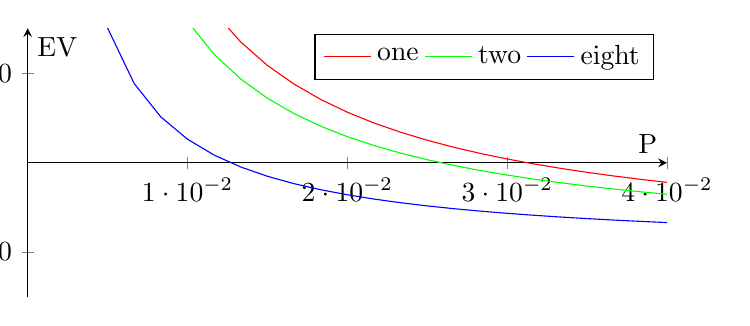
\begin{tikzpicture}[trim axis left]
			\begin{axis}[consensusAxisEvStyle, xtick distance=0.01, xmax = 0.04]
				\addplot[color=red,domain=0:0.04]{(0.04 * 100 / (359 * 1 + 100)) * (359 / x) * (1 + 0) - 100};
				\addlegendentry{one}

				\addplot[color=green,domain=0:0.04]{(0.04 * 100 / (359 * 1 + 2 * 100)) * (359 / x) * (1 + 1 * 100 * x / 359) - 100};
				\addlegendentry{two}

				\addplot[color=blue,domain=0:0.04]{(0.04 * 100 / (359 * 1 + 8 * 100)) * (359 / x) * (1 + 7 * 100 * x / 359) - 100};
				\addlegendentry{eight}
			\end{axis}
		\end{tikzpicture}
	}{Fee attack declining with more attackers (F = 100, $\bar{F} = 1$)}
\end{figure}
